\documentclass[tikz,border=4pt]{standalone}
\usepackage{amsmath}
\usepackage{xcolor}
\usepackage{tikz}
\usepackage{pgfplots}
\pgfplotsset{compat=1.18}

\definecolor{caraprimary}{RGB}{30,60,120}
\definecolor{caraaccent}{RGB}{200,80,60}

\begin{document}
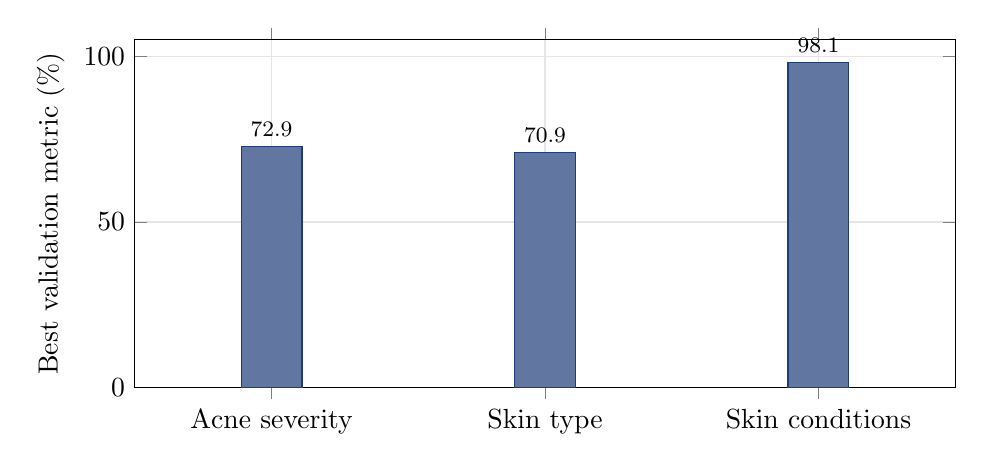
\begin{tikzpicture}
\begin{axis}[
    ybar,
    width=12cm, height=6cm,
    bar width=22pt,
    ymin=0, ymax=105,
    symbolic x coords={Acne severity, Skin type, Skin conditions},
    xtick=data,
    ylabel={Best validation metric (\%)},
    nodes near coords,
    nodes near coords style={font=\footnotesize},
    enlarge x limits=0.25,
    grid=both, grid style={gray!20},
]
\addplot[fill=caraprimary!70, draw=caraprimary] coordinates {
    (Acne severity, 72.9)
    (Skin type,     70.9)
    (Skin conditions,   98.1)
};
\end{axis}
\end{tikzpicture}
\end{document}
